
\documentclass[10pt]{beamer}
\usepackage{amsmath}
\usepackage{mathtools}
\usepackage{multimedia}
\usepackage{hyperref}


\usefonttheme{professionalfonts} % using non standard fonts for beamer
\usefonttheme{serif} % default family is serif
%\documentclass[12pt]{beamerthemeSam.sty}
\usepackage{epsf}
%\usepackage{pstricks}
%\usepackage[orientation=portrait,size=A4]{beamerposter}
\geometry{paperwidth=160mm,paperheight=120mm}
%DT favorite definitions
\def\LL{\left\langle}	% left angle bracket
\def\RR{\right\rangle}	% right angle bracket
\def\LP{\left(}		% left parenthesis
\def\RP{\right)}	% right parenthesis
\def\LB{\left\{}	% left curly bracket
\def\RB{\right\}}	% right curly bracket
\def\PAR#1#2{ {{\partial #1}\over{\partial #2}} }
\def\PARTWO#1#2{ {{\partial^2 #1}\over{\partial #2}^2} }
\def\PARTWOMIX#1#2#3{ {{\partial^2 #1}\over{\partial #2 \partial #3}} }

\def\rightpartial{{\overrightarrow\partial}}
\def\leftpartial{{\overleftarrow\partial}}
\def\diffpartial{\buildrel\leftrightarrow\over\partial}

\def\BC{\begin{center}}
	\def\BS{\bigskip}
\def\EC{\end{center}}
\def\BCC{\begin{columns}}
\def\ECC{\end{columns}}
\def\HC{\column{0.5\textwidth}}	
\def\TC{\column{0.33\textwidth}}	
\def\BN{\begin{enumerate}}
\def\EN{\end{enumerate}}
\def\BI{\begin{itemize}}
\def\EI{\end{itemize}}
\def\BE{\begin{displaymath}}
\def\EE{\end{displaymath}}
\def\BEA{\begin{eqnarray*}}
\def\EEA{\end{eqnarray*}}
\def\BNEA{\begin{eqnarray}}
\def\ENEA{\end{eqnarray}}
\def\EL{\nonumber\\}

\newcommand{\etal}{{\it et al.}}
\newcommand{\gbeta}{6/g^2}
\newcommand{\la}[1]{\label{#1}}
\newcommand{\ie}{{\em i.e.\ }}
\newcommand{\eg}{{\em e.\,g.\ }}
\newcommand{\cf}{cf.\ }
\newcommand{\etc}{etc.\ }
\newcommand{\atantwo}{{\rm atan2}}
\newcommand{\Tr}{{\rm Tr}}
\newcommand{\dt}{\Delta t}
\newcommand{\op}{{\cal O}}
\newcommand{\msbar}{{\overline{\rm MS}}}
\def\chpt{\raise0.4ex\hbox{$\chi$}PT}
\def\schpt{S\raise0.4ex\hbox{$\chi$}PT}
\def\MeV{{\rm Me\!V}}
\def\GeV{{\rm Ge\!V}}

%AB: my color definitions
%\definecolor{mygarnet}{rgb}{0.445,0.184,0.215}
%\definecolor{mygold}{rgb}{0.848,0.848,0.098}
%\definecolor{myg2g}{rgb}{0.647,0.316,0.157}
\definecolor{A}{rgb}{1.0,0.3,0.3}
\definecolor{B}{rgb}{0.0,1.0,0.0}
\definecolor{C}{rgb}{1.0,1.0,0.0}
\definecolor{D}{rgb}{0.5,0.5,1.0}
\definecolor{E}{rgb}{0.7,0.7,0.7}
\definecolor{abtitlecolor}{rgb}{1.0,1.0,1.0}
\definecolor{absecondarycolor}{rgb}{0.0,0.416,0.804}
\definecolor{abprimarycolor}{rgb}{1.0,0.686,0.0}
\definecolor{Red}           {rgb}{1,0.4,0.4}
\definecolor{Yellow}           {rgb}{1,1,0.0}
\definecolor{Grey}          {cmyk}{.7,.7,.7,0}
\definecolor{Blue}          {cmyk}{1,1,0,0}
\definecolor{Green}         {cmyk}{1,0,1,0}
\definecolor{Brown}         {cmyk}{0,0.81,1,0.60}
\definecolor{Silver}        {rgb}{0.95,0.9,1.0}
\definecolor{Sky}           {rgb}{0.07,0.0,0.2}
\definecolor{Darkbrown}     {rgb}{0.4,0.3,0.2}
\definecolor{40Gray}        {rgb}{0.4,0.4,0.5}
\usetheme{Madrid}


\setbeamercolor{normal text}{fg=Silver,bg=Sky}

%AB: redefinition of beamer colors
%\setbeamercolor{palette tertiary}{fg=white,bg=mygarnet}
%\setbeamercolor{palette secondary}{fg=white,bg=myg2g}
%\setbeamercolor{palette primary}{fg=black,bg=mygold}
\setbeamercolor{title}{fg=abtitlecolor}
\setbeamercolor{frametitle}{fg=abtitlecolor}
\setbeamercolor{palette tertiary}{fg=white,bg=Darkbrown}
\setbeamercolor{palette secondary}{fg=white,bg=absecondarycolor}
\setbeamercolor{palette primary}{fg=white,bg=40Gray}
\setbeamercolor{structure}{fg=abtitlecolor}

\setbeamerfont{section in toc}{series=\bfseries}

%AB: remove navigation icons
\beamertemplatenavigationsymbolsempty
\title[Keeping time]{
  \textbf {Keeping time}
}

\author [Astronomy 101]{Astronomy 101\\Syracuse University, Fall 2021\\Walter Freeman}

\date{\today}

\begin{document}



\frame{\titlepage}

\frame{
	
\it
	And that inverted Bowl we call The Sky,\\
	Whereunder crawling coop't we live and die,\\
	Lift not thy hands to it for help -- for It\\
	Rolls impotently on as Thou or I.
\rm	
	\begin{flushright}--Omar Khayyám (1048-1131), translated into English by Edward FitzGerald (1859) \end{flushright}
\bigskip
\bigskip
\bigskip	
\it	
	I'm cheating death\\
	In Stellarium\\
	I'm peeking ahead\\
	To stars I will never see.
\rm	
	\begin{flushright}--Poetic text message from K. Alice Lindsay, used with permission\end{flushright}
}

\frame{
\BC

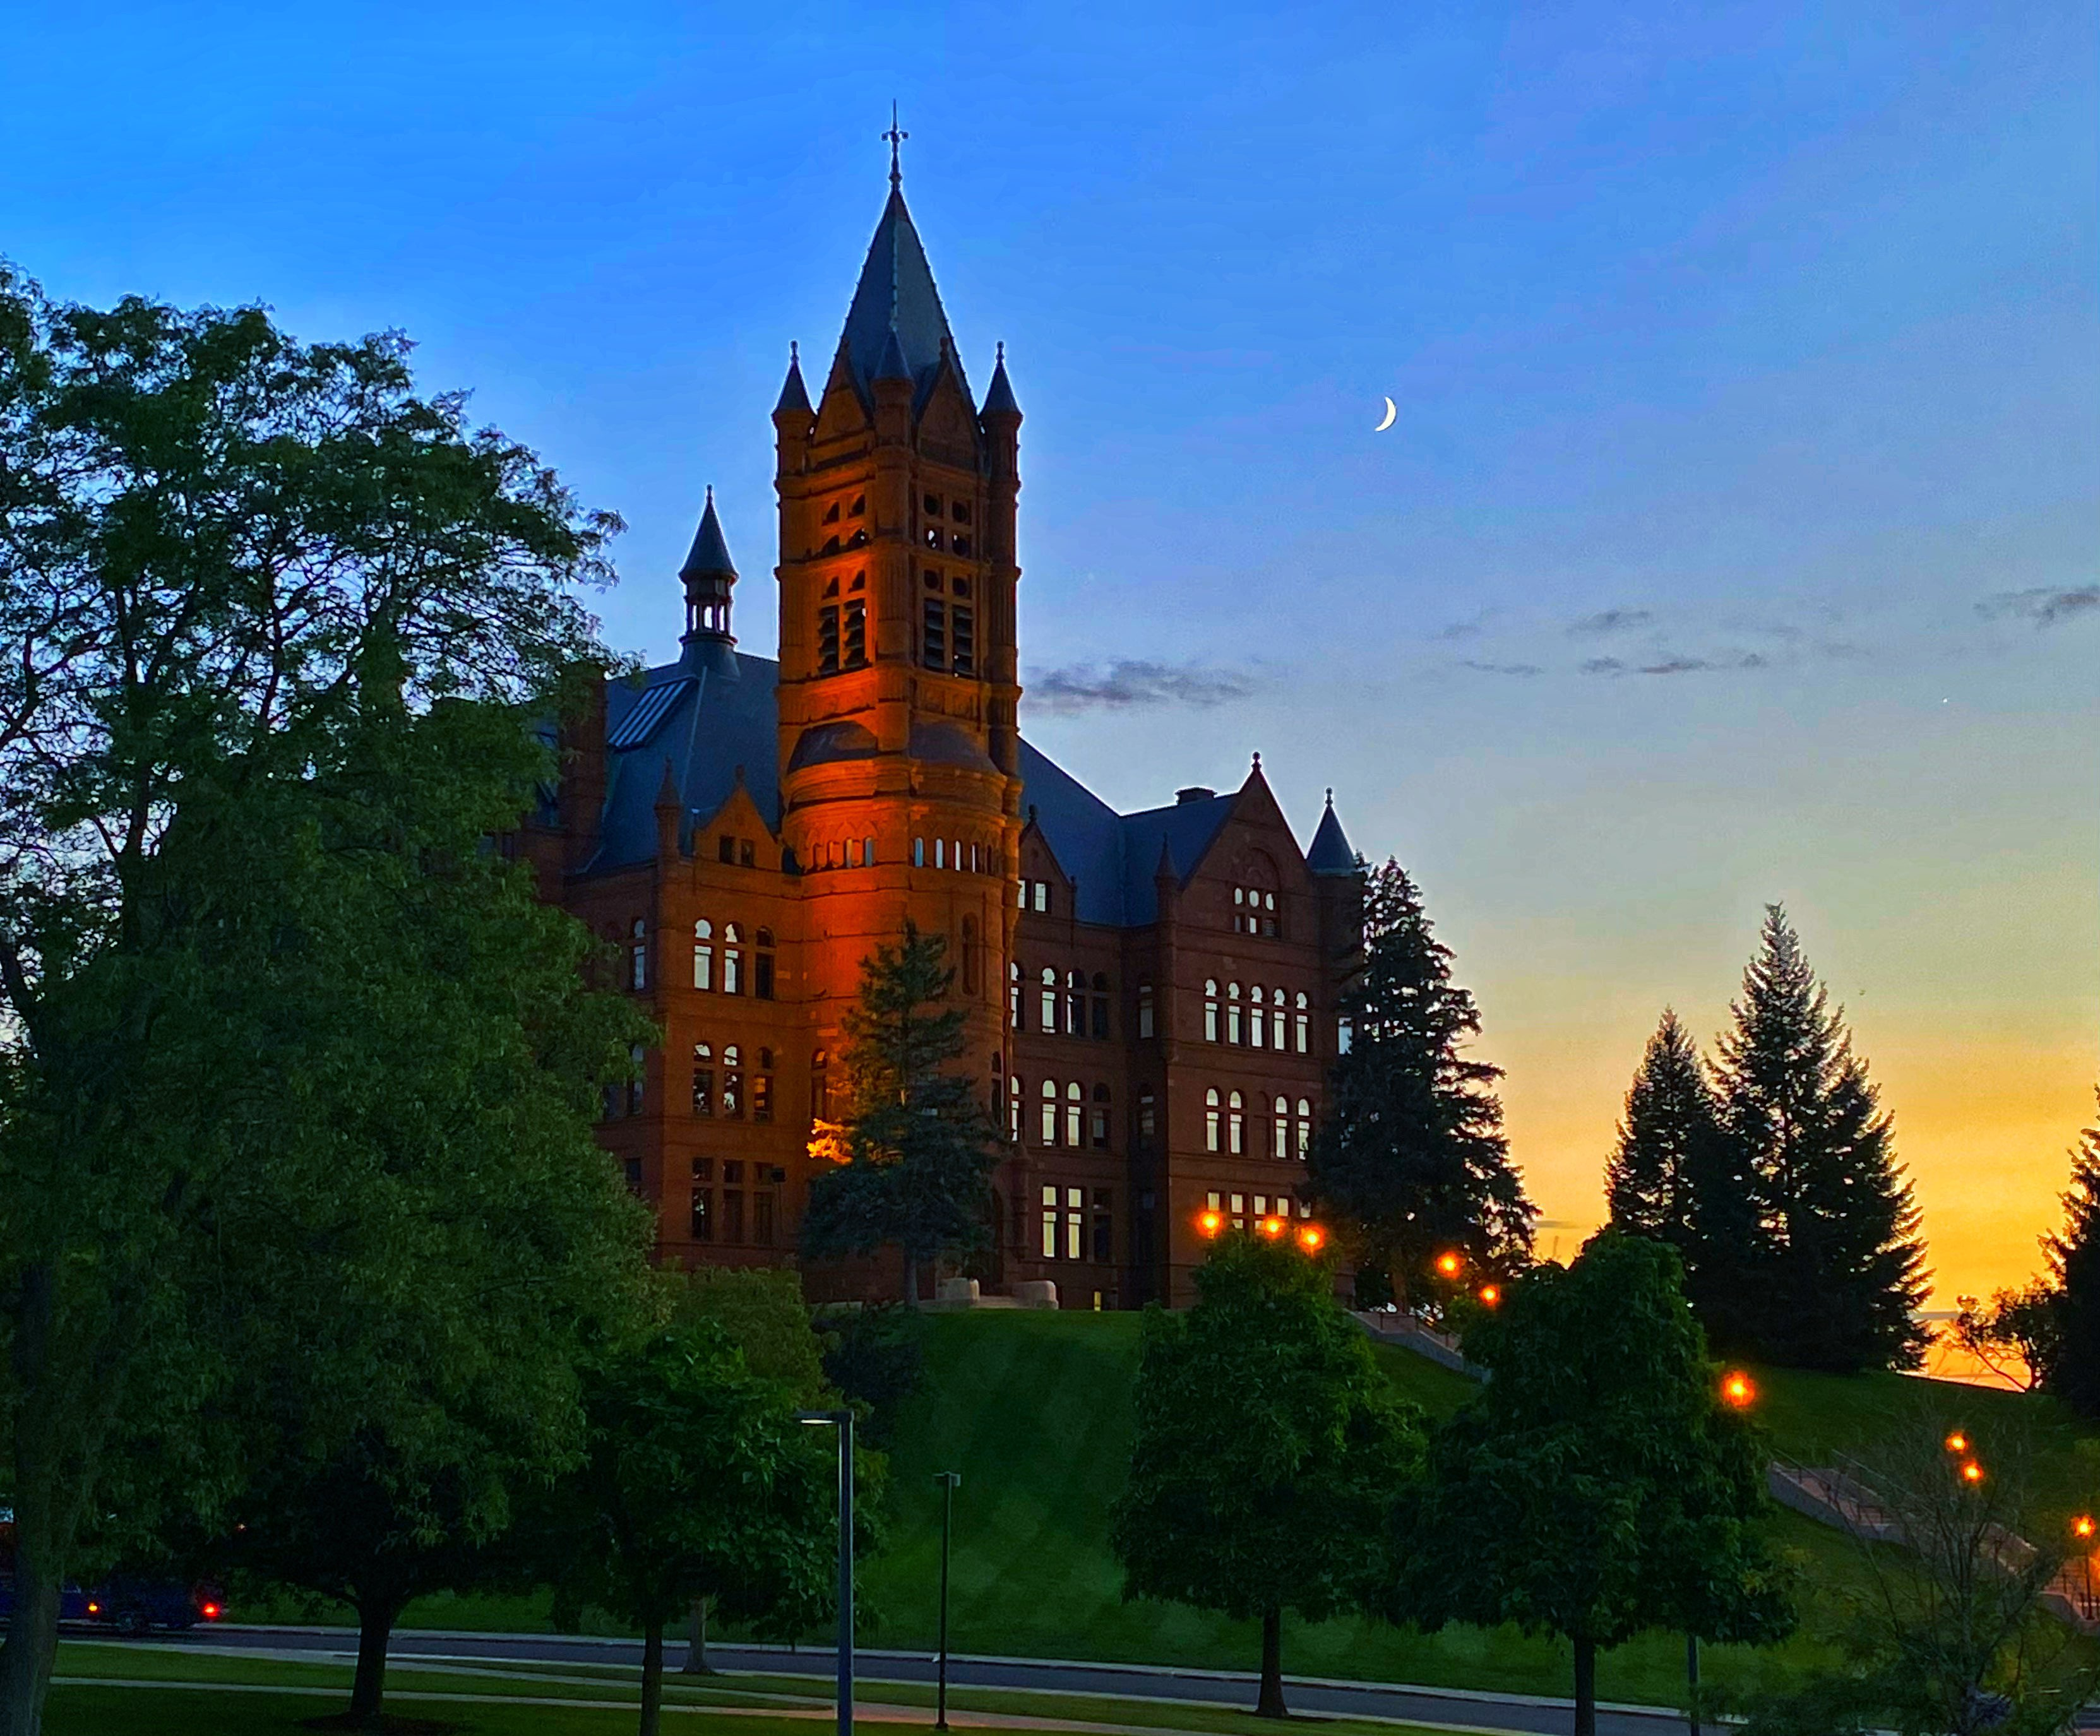
\includegraphics[width=4.5in]{moon-crouse.jpg}

\it \footnotesize The crescent moon and Venus at sunset by Crouse College, by Astronomy 101 student ComradeWilhelm (Discord alias)

\EC 

}

\frame{\frametitle{Announcements}
	\Large
	
	\begin{itemize}
		\item Our printers are back alive. Prelab 4 will be available in the Physics Clinic by 5pm today.
		\item Quiz 1+2 is Tuesday:
		\begin{itemize}
			\item We will post seating charts and send them out as PDF's ahead of time this time
			\item Please bring a pencil and knowledge of your SUID
		\end{itemize}
	
	\BS
	
	\item Blackboard is having trouble; I have your scores on Quiz 1 and will post them tomorrow once Blackboard is working again
	\end{itemize}
	
	
}
	
	\frame{\frametitle{\textbf{Writing assignment}}
		\Large \BC The full thing is on the website. In brief:\EC
		
		\BI
		\item Choose a historical calendar
		\item Research it
		\item Write on how it connects timekeeping to the cycles in the sky
		\item Due in three weeks (October 18)
		\item Potential for significant extra credit
		\item Some special assignments for particular calendars; read the whole thing
		\EI
	}
	
	

\frame{\frametitle{\textbf{A past test question}}
	
	In {\it The Lord of the Rings}, Frodo and Sam traveled with Sm\'{e}agol to Mordor. During part of their journey, they needed to hide from the Nazg\^{u}l, so they could only travel during absolute darkness -- when neither the Sun nor the Moon were visible in the sky.
	
	\bigskip
	
	If the Moon was waxing gibbous, during what part of the day could they travel?
	
	\Huge
	
	
	
	\bigskip
	\bigskip
	\bigskip
	
	\color{A}A: For a short time after sunset \\
	\color{B}B: For a short time before sunrise \\
	\color{C}C: During the first half of the night \\
	\color{D}D: During the last half of the night \\ \pause
	\color{E}E: What's moonlight, precioussss? \\ 
}

\frame{\frametitle{\textbf{Unpredictable things in the sky}}
	\Large
	\BC
	Why are the changes in the seasons in {\it Game of Thrones} so terrifying?
	\EC
	
	\pause
	\bigskip
	\bigskip
	\bigskip
	
	... they're unpredictable!
	
	\bigskip
	
	We've long used the immutability of the sky as a symbol for constancy. The cycles of the Sun, Moon, and stars don't ever change, but some things do!
	
	\bigskip
	
	These unexpected things in the sky once terrified people; now we know why they happen.
}
\frame{\frametitle{\textbf{Eclipses}}
	\large
	You know that during a new moon, the Moon lies roughly between the Earth and the Sun.
	
	\bigskip
	
	However, the Moon's orbit is tilted just a bit, so it usually passes over or under the Sun.
	
	\bigskip
	
	\BC 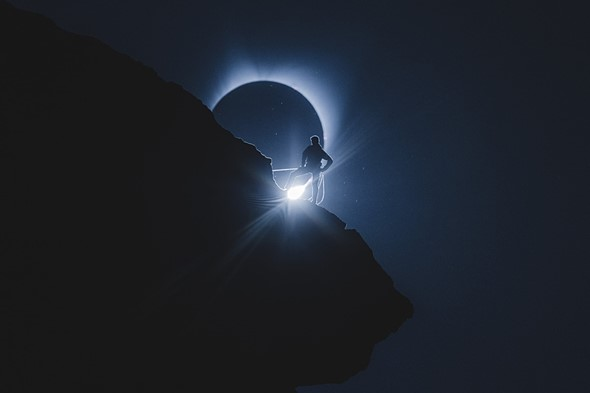
\includegraphics[width=0.6\textwidth]{viralclimber1.jpeg}\EC
	
	\bigskip
	\BC
	If it passes in front, you get a solar eclipse!
	
	This terrified many of the ancients -- ``the Sun got eaten! We're doomed!''
	\EC
}

\frame{\frametitle{\textbf{Eclipses}}
	\Large
	You know that during a full moon, the Earth lies roughly between the Moon and the Sun.
	
	\bigskip
	\bigskip
	\bigskip
	
	Same deal: usually the Earth's shadow misses the Moon. Sometimes it doesn't!
	
	\bigskip
	
	\BC 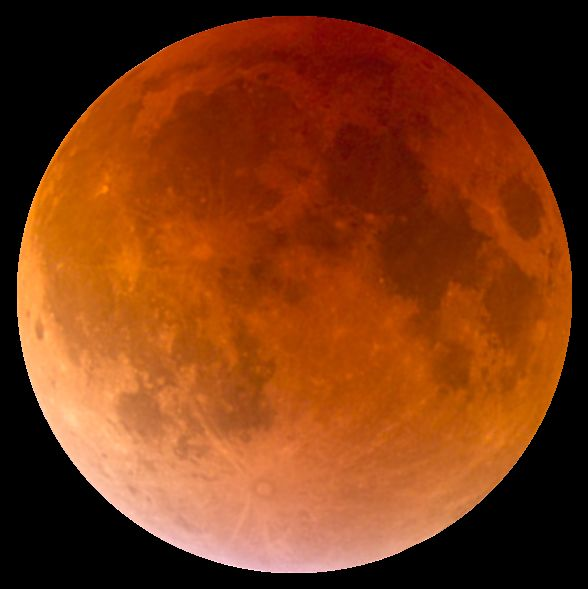
\includegraphics[width=0.27\textwidth]{lunar-eclipse.jpg}\EC
	
	\bigskip
	
	\large
	
	Here some light is refracted by the atmosphere. The blue component is scattered away by the atmosphere; the red component bends and hits the Moon.
	
}
\frame{\frametitle{\textbf{Meteors}}
	
	\large
	
	Orbits of things in the Solar System are not always close to circular.
	
	\bigskip
	
	There are lots of small things in the Solar System, many of which have elongated orbits that sometimes cross ours.
	
	\bigskip
	
	Meteors:
	
	\large
	
	\begin{columns}
		\column{0.6\textwidth}
		
		\BI
		\item{Little rocky or metallic bits of matter that orbit the Sun}
		\item{Sometimes they get to Earth and glow as atmospheric drag heats them}
		\item{Sometimes they hit the surface, and we get chunks of space-slag}
		\item{Historical cultures sometimes used them as easy access to metal}
		\EI
		\column{0.4\textwidth}
		\BC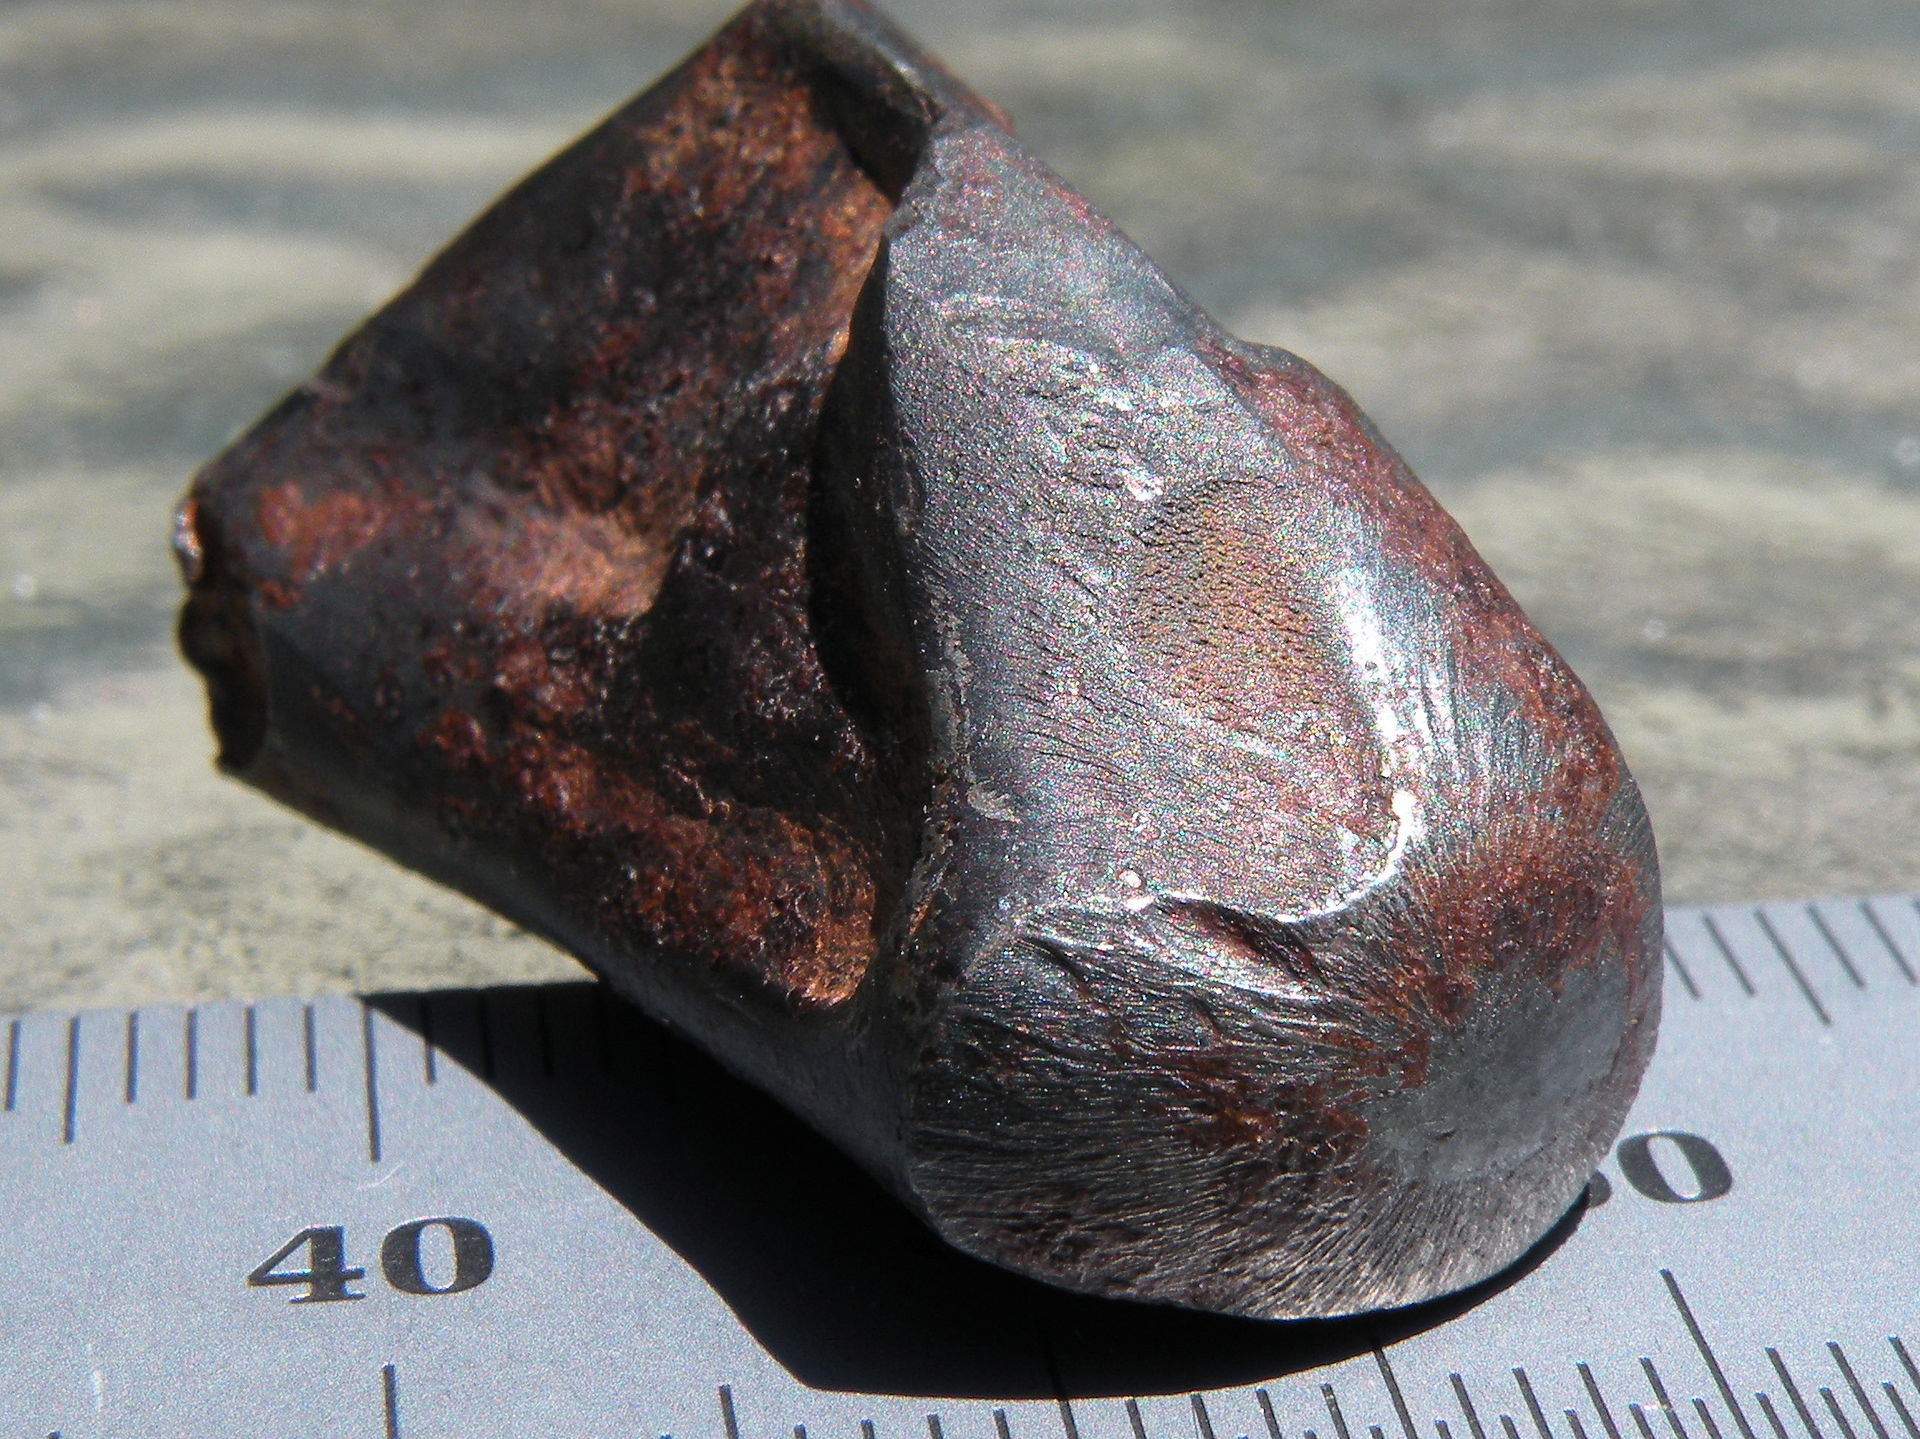
\includegraphics[width=\textwidth]{meteorite.jpg}\EC
	\end{columns}
}
\frame{\frametitle{\textbf{Comets}}
	
	\Large
	
	Comets are ``dirty snowballs'' whose orbits are {\it highly} elongated.
	
	\large
	
	\begin{columns}
		\column{0.6\textwidth}
		
		\BI
		\item{Mostly made of ice}
		\item{When they get close to the Sun, the heat melts bits off of them}
		\item{This stream of stuff reflects sunlight and makes the comet's ``tail''}
		\item{Historical cultures were often terrified of them, but they're just space-snowballs}
		\EI
		\column{0.4\textwidth}
		\BC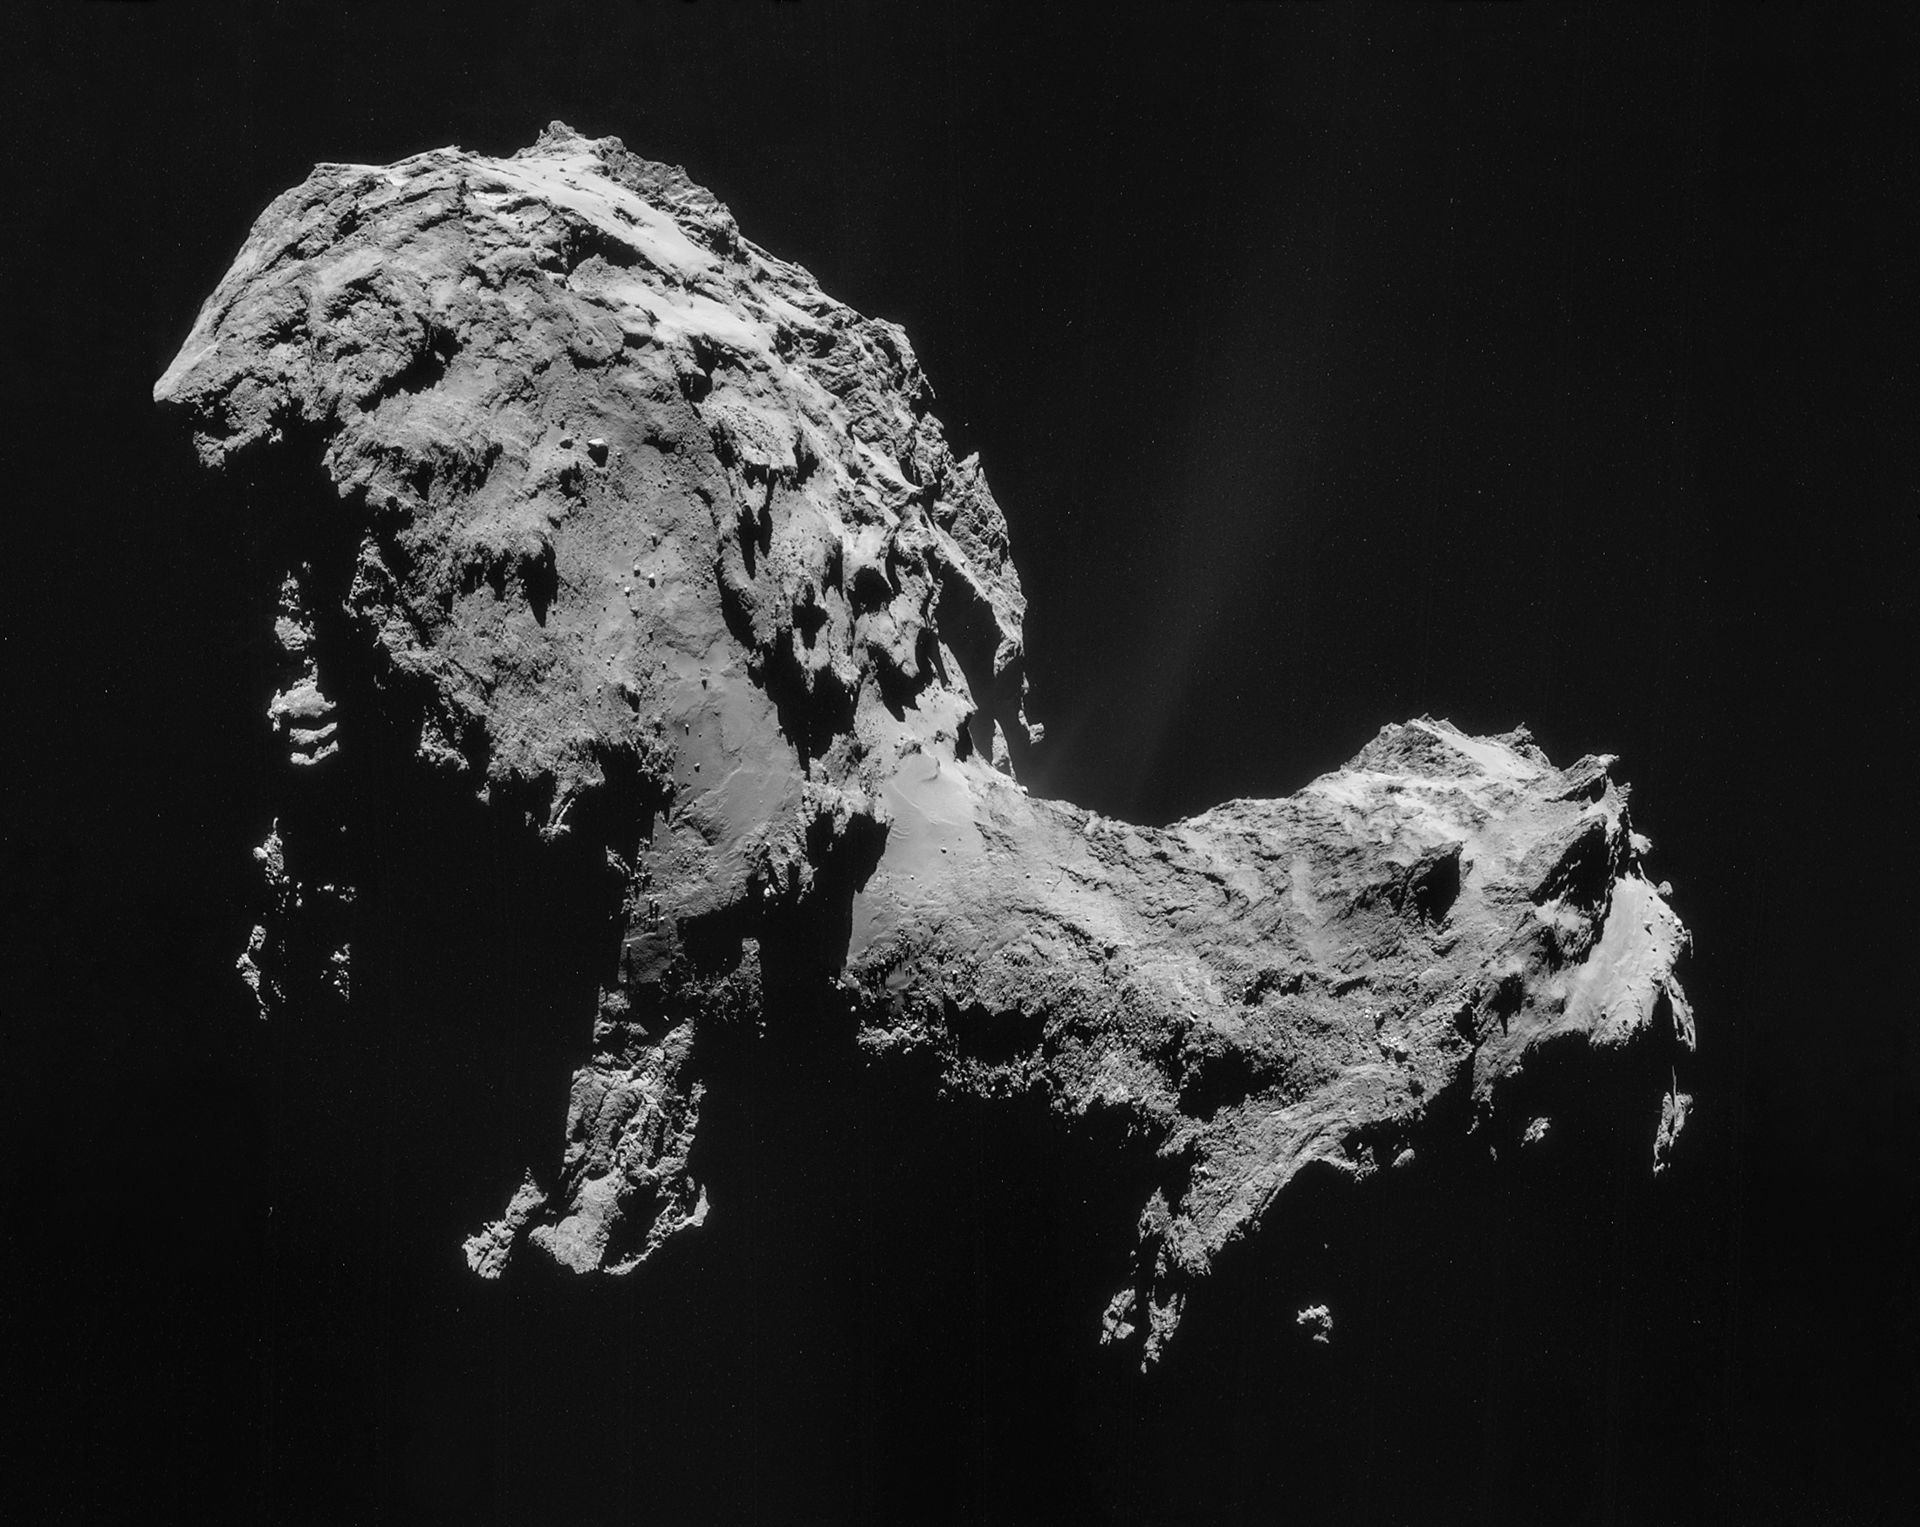
\includegraphics[width=\textwidth]{comet-rosetta.jpg}\EC
	\end{columns}
}



\frame{\frametitle{\textbf{The planets: semi-predictable}}
	
	\Large
	\BC
	Demo on {\it Stellarium}
	\EC
	
	\pause
	\bigskip
	
	
	Sometimes some planets appear to go backwards (``retrograde motion'').
	
	\bigskip
	\bigskip
	
	\large
	
	This tells us that celestial sphere model can't be literally true. Why does it work for everything else?
	
	\BI
	\item{The celestial sphere model works if things appear to only rotate around the Earth.}
	\item{The stars are so far away that only the Earth's rotation matters}
	\item{The Earth orbits the Sun, so we just pretend that the Sun is on a different sphere turning a bit slower, taking into account both our revolution around it and our rotation}
	\item{The Moon orbits the Earth, so we again put the Moon on a different sphere, turning slower}
	\item{... but how can we get a sphere to go forwards and backwards?}
	\item{\bf The celestial sphere model gets the motion of the planets badly wrong}
	\EI
}

%
%\frame{\frametitle{\textbf{Announcements}}
%\large
%\BI
%\item Project 1 is due tomorrow at midnight
%\item Submission instructions are on the groups page
%\item Lots of discussion on Piazza and at my help hours
%\item More discussion hours: tomorrow, 10am-noon on the steps of Hendricks
%\EI
%}

%\frame{\frametitle{\textbf{Announcements and questions}}
%	
%	\large
%	\BI
%	\item Remember, your evaluations for Project 1 are due by midnight tonight (or three days after you received the project from the submitting group, if they were late)
%	\item Project 2 has been written; will be posted today after class
%	\item This will also include updated group rosters
%	\EI
%	
%	\BS\BS\BS
%	
%	Please make an effort to work with your groupmates as adults. If you're having issues still after Lab 2, we will reassign you. 
%	
%}
%	
%
%
%
%
%\frame{
%	\begin{columns}
%		\column{0.7\textwidth}
%		\BC
%		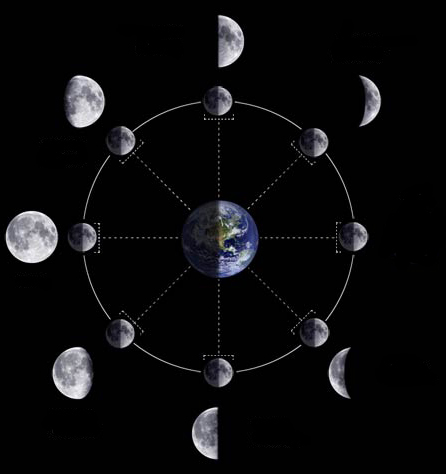
\includegraphics[width=0.95\textwidth]{phases.jpg}
%		\EC
%		\column{0.3\textwidth}
%		\large
%		You can figure all of this out by drawing pictures.
%		
%		\bigskip
%		\bigskip
%		\bigskip
%		
%		{\bf \color{Red}Do this} whenever you need to figure something out about the Moon...
%		
%		\bigskip
%		\bigskip
%		\bigskip
%		
%		Let's make a doodle on the board and see how much we can figure out...
%		
%	\end{columns}
%}

%\frame{
%	
%	\Large
%	
%	When the full moon is high in the sky, what time of day is it?	
%	
%	\vspace{2in}
%	
%}
%
%\frame{
%	
%	\Large
%	
%	What phase of the moon is mostly seen during the day?
%	\vspace{2in}
%	
%}
%
%
%
%\frame{
%	
%	\large
%	
%	When the waxing half moon is just rising over the horizon, what time of day is it?
%	\vspace{2in}
%
%}
%
%\frame{
%	
%	\large
%	
%	As seen in the Northern Hemisphere, which part of a waning crescent moon will be lit?
%	
%	\pause \bigskip
%	
%	What about the Equator?
%	
%	
%}

\frame{\frametitle{\textbf{Keeping time: the very predictable}}
	
	\large
	
	The predictable cycles in the sky are the basis for the way we keep time.
	
	\begin{columns}
		\column{0.33\textwidth}
		\color{Yellow}
		\begin{center}
			\Large One day
		\end{center}
	\small
	\BI
	\item Earth rotating around its axis 
	\EI
		\column{0.33\textwidth}
		\color{B}
		\BC
		\Large One year
		\EC
			\small
		\BI
		\item 365 days
		\item Earth's orbit around the Sun
		\EI
		\pause
		
		\column{0.33\textwidth}
		\Large
		\color{D}
		\BC
		One month
		\EC
		
			\small
		\BI
		\item One orbit of the Moon around the Earth 
		\EI
		
	\end{columns}

\vspace{2in}
}

%
%\frame{\frametitle{\textbf{Solar and sidereal days}}
%	
%	\large
%	
%	Is one day...
%	
%	\BI
%	\item ... the amount of time it takes Earth to rotate once?
%	\item ... the amount of time between noon one day and noon the next day?
%	\item ... something else!
%	\EI
%	
%	\pause\BS
%	
%	There are {\it two kinds of day}. Let's see why they are different on the board.
%	
%	\BS\pause
%	
%	
%	
%	
%	\BI
%	\item \color{A} One {\it solar day:} judged by the apparent motion of the Sun: from noon to noon
%	\item \color{B} One {\it sidereal day:} judged by the apparent motion of the stars: Earth, and the celestial sphere, rotate exactly $360^\circ$
%	\EI
%	
%	\BS
%	
%	Which one is more important for our lives?
%}
	
\frame{\frametitle{\textbf {A reminder: Two sorts of day}}
	\large
	The {\it sidereal day} is the amount of time it takes the Earth, and thus the celestial sphere, to rotate once.
	
	\bigskip
	
	\BC     {\color{Red} One sidereal day $\rightarrow$ $360^\circ$ rotation of the Earth}\EC
	
	\bigskip
	\bigskip
	The {\it solar day} is the amount of time from solar noon to solar noon.
	
	\bigskip
	
	Since the Earth orbits the Sun, this requires more than $360^\circ$ rotation:
	\BI
	\item{$360^\circ$ plus a little extra, to compensate for the motion of the Earth around the Sun}
	\item{In my animation, with the ``fast orbit'', this is a lot more than $360^\circ$}
	\item{In the real world, the Earth moves only 1/365 $\approx$ $1^\circ$ around the Sun each day}
	\item{... so in a solar day the Earth rotates:}
	\begin{itemize}
		\item $360^\circ$ for the stars to rise and set once...
		\item ... plus {\it one more degree} to compensate for the Earth's movement
	\end{itemize}
	
	
	
	\EI
	\BC     {\color{B} One solar day $\rightarrow$ $361^\circ$ rotation of the Earth}    \EC
	
}

\frame{
	
	\begin{columns}
		\column{0.5\textwidth}
		\color{B}
		\begin{center}
			\Large                  Solar day:
		\end{center}
		\begin{itemize}
			\normalsize
			\item $361^\circ$ rotation of Earth
			\item The Sun returns to its same position (east/west)
			\item A bit more than a sidereal day $\rightarrow$ the stars move ``too far''
			\color{B}\item Exactly 24 hours
		\end{itemize}
		\column{0.5\textwidth}
		\color{Red}
		\begin{center}
			\Large                  Sidereal day:
		\end{center}
		\begin{itemize}
			\normalsize
			\item $360^\circ$ rotation of Earth
			\item The stars return to their same positions (exactly)
			\item A bit less than a solar day $\rightarrow$ the Sun moves ``too little''
			\color{A}\item Four minutes less than 24 hours
		\end{itemize}
	\end{columns}

\large

}

\frame{\frametitle{\textbf{What about the moonth?}}
	
	Is a lunar month...
	
	\BI
	\item One complete cycle of phases of the Moon? (new moon to new moon)
	\item One orbit of the Moon around the Earth?
	\EI
	
	\BS\pause
	
	Same deal:
	\BI
	\item \color{A} Synodic month: One complete cycle of phases of the Moon (29.5 days)
	\item \color{B} Sidereal month: One orbit of the Moon (``Moon in Libra $\rightarrow$ Moon in Libra'' -- 27.3 days)
	\pause
	\item \color{C} Calendar month -- it varies depending on the calendar!
	\EI
}

\frame{\frametitle{\textbf{What about the year?}}
	
	Is a year...
	
	\BI
	\item ... from winter solstice to winter solstice?
	\item ... One orbit of the Earth around the Sun? (``Sun in Sagittarius $\rightarrow$ Sun in Sagittarius'')
	\EI
	
	\pause
	
	\color{C}What would have to happen for them to be different?
	
	
	\BS\pause\BS\BS
	
	The orientation of the Earth's tilt makes one rotation every 26,000 years.
	
	\BS
	
	Same deal:
	\BI
	\item \color{A} Tropical (seasonal) year: solstice to solstice
	\item \color{B} Sidereal year: one orbit around the Sun; 1/26,000 less than a seasonal year
	\EI
}

\frame{\frametitle{\textbf{Now what do we have?}}

\BCC

\TC \BC \color{A} \huge The year \EC 
\TC \BC \color{B} \huge The day \EC 
\TC \BC \color{C} \huge The moonth \EC 
	
	\ECC
	
	\BCC
	
	
\TC \BC \color{A} \large Sidereal year \EC 
\TC \BC \color{B} \large Sidereal day \EC 
\TC \BC \color{C} \large Sidereal moonth \EC 
	
	
\ECC

\BCC

\TC 

\BI
\small \color{A}
\item One Earth orbit around Sun
\item 365.26 24-hour days (1/26,000 {\it more} than a seasonal year)
\item Sun returns to same place relative to stars
\EI

\TC 

\BI
\small \color{B}
\item One Earth rotation
\item 23 hours 56 minutes (1/365 {\it less} than a solar day)
\item Stars return to the same places in the sky
\EI


\TC 

\BI
\small \color{C}
\item One Moon orbit around Earth
\item 27.3 days (about 1/12 {\it less} than a synodic moonth)
\item Moon returns to same place relative to stars
\EI

\ECC

\pause	
	
		
	\BCC
	
	
	\TC \BC \color{A} \large Seasonal year \EC 
	\TC \BC \color{B} \large Solar day \EC 
	\TC \BC \color{C} \large Synodic moonth \EC 
	
	
	\ECC
	
	\BCC
	
	\TC 
	\BI
	\small \color{A}
	\item One cycle of the seasons (solstice to solstice) 
	\item 365.24 24-hour days (1/26,000 {\it less} than a sidereal year)
	\item Sun does not quite return to same place relative to stars!
	\EI
	
	\TC 
	\BI
		\small \color{B}
	\item Noon to noon / midnight to midnight
	\item 24 hours (1/365 {\it more} than a sidereal day)
	\item Stars do not return to the same places in the sky
	
	\EI
	
	
	\TC 
	\BI
		\small \color{C}
	\item One cycle of the Moon phases
	\item 29.5 days (about 1/12 {\it more} than a sidereal moonth)
	\item Moon returns to same place relative to stars
	
	\EI
	
	\ECC
}

\frame{\frametitle{\textbf{Now what do we have?}}
	
	\BCC
	
	\TC \BC \color{A} \huge The year \EC 
	\TC \BC \color{B} \huge The day \EC 
	\TC \BC \color{C} \huge The moonth \EC 
	
	\ECC
	
	\BCC
	 \color{Grey}
	
	\TC \BC \large Sidereal year \EC 
	\TC \BC  \large Sidereal day \EC 
	\TC \BC \large Sidereal moonth \EC 
	
	
	\ECC
	
	\BCC
	
	\TC 
	
	\BI
	\small
	\color{Grey}
	\item One Earth orbit around Sun
	\item 365.26 24-hour days 
	\item Sun returns to same place relative to stars
	\EI
	
	\TC 
	
	\BI
	\small \color{Grey}
	\item One Earth rotation
	\item 23 hours 56 minutes 
	\item Stars return to the same places in the sky
	\EI
	
	
	\TC 
	
	\BI
	\small \color{Grey}
	\item One Moon orbit around Earth
	\item 27.3 days 
	\item Moon returns to same place relative to stars
	\EI
	
	\ECC
	
	
	
	\BCC
	
	
	\TC \BC \color{A} \large Seasonal year \EC 
	\TC \BC \color{B} \large Solar day \EC 
	\TC \BC \color{C} \large Synodic moonth \EC 
	
	
	\ECC
	
	\BCC
	
	\TC 
	\BI
	\small \color{A}
	\item One cycle of the seasons (solstice to solstice) 
	\item 365.24 24-hour days 
	\item Sun does not quite return to same place relative to stars!
		\EI
	
	
	\TC 
	\BI
	\small \color{B}
	\item Noon to noon / midnight to midnight
	\item 24 hours 
	\item Stars do not return to the same places in the sky
	\EI

	
	\TC 
	\BI
	\small \color{C}
	\item One cycle of the Moon phases
	\item 29.5 days
	\item Moon returns to same place relative to stars
	\EI
	
	\ECC

\vspace{0.2in}		
	
	\BCC


	
\TC	\small Difference caused by wobble of Earth's axis;
	seasonal year about 1/26,000 shorter
	
	\TC	\small Difference caused by motion of Earth around Sun: solar day about 1/365 longer
	
	\TC	\small Difference caused by motion of Earth and Moon around Sun:
	synodic moonth about 1/12 longer
	\ECC
}

\frame{\frametitle{\textbf{Keeping time}}
	\large
	
	How many solar days are in a seasonal year?
	
	\BS\pause
	
	
	How many synodic moonths are in a seasonal year?
	
	\BS\pause
	
	How many solar days are in a moonth?
}


\frame{\frametitle{\textbf{Building a calendar}}
	\large
	\color{E}
	How many solar days are in a seasonal year?

\color{A} 365.24 (ack, doesn't come out even)
	
	\BS\pause
	\color{E}
	How many synodic moonths are in a seasonal year?
	
\color{B} 364.24 / 29.5 = 12.35 (also doesn't come out even)
	
	\BS\pause
	
	\color{E}
	
	How many solar days are in a moonth?
	
	\color{C} 29.5 (ack, doesn't come out even)
	
	\BS

	\color{D}
	... what do we do?	
	\pause
		Two choices:
	
	\BI
	\item Don't worry about it (Gregorian months aren't lined up with the moonths)\pause
	\item Intercalation: add extras (about one in four years is a leap year)
	\EI
}


\end{document}

